\chapter{Gesamtintegration}
%\section{Programmaufbau}
%\begin{figure}[h]
%	\centering
%	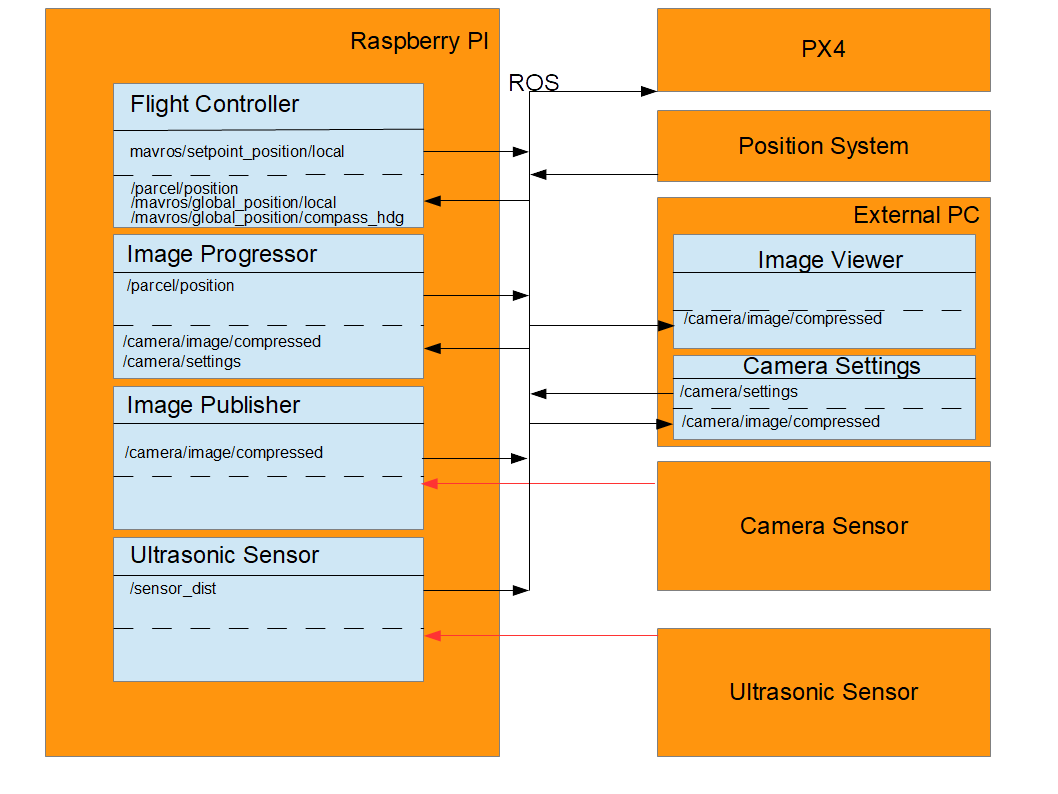
\includegraphics[scale=0.5]{"Grafiken/Nodes.png"}
%	\caption{Programmaufbau}
%	\label{fig:meine-grafik}
%\end{figure}
%Das Programm besteht grundlegend aus 4 Nodes/Unterprogrammen. Zum einen dem Image Publisher und Ultrasonic Sensor. Und zum anderen aus dem Image Progressor und Flight %Controller, um diese Daten zu verarbeiten. In der obigen Grafik sind diese Nodes, sowie deren empfangene(unten) und gesendete(oben) Themen zu sehen. \\
%\\
%Alle 4 Nodes laufen gleichzeitig und kommunizieren über das Interface ROS(siehe Interfaces). Um Multithreading(ein paralleles ablaufen der Unterprogramme) zu gewährleisten, wird jedes Programm in einem separaten Thread ausgeführt.\\
%\\
%Grundlegend sind alle Programme gleich aufgebaut. Zuerst gibt es einen Teil, der die Verbindung zum ROS Interface herstellt. Dafür wird zuerst gewartet, bis der Server läuft, anschließend werden die entsprechenden Themen deklariert. Nun geht das Programm in eine Schleife, bei der es auf eine ankommende Nachricht wartet. Empfängt es eine Nachricht, so verarbeitet es diese. Gegenbefalls sendet es regelmäßig eine neue Nachricht. Der Server auf dem diese Themen laufen, wird dabei vom Raspberry Pi gehostet. Sobald dieser steht, können alle Nodes zu spezifischen Themen Nachrichten senden oder die gesendeten Nachrichten zu diesen Themen empfangen.\\
%\\

\section{Sensordatenverarbeitung}
Prinzipiell gibt es 3. Sensoren. Zum einen der Ultraschallsensor, um die Höhe genau und jederzeit bestimmen zu können. Außerdem gibt es einen Kamerasensor, um die Position des Paketes zu bestimmen. Das dritte Sensorsystem ist da, um die Position der Drohne zu bestimmen. Dieses wird vom Institut für Technische und Numerische Mechanik gestellt. Es ist für das fliegen der Drohne existenziell wichtig.\\
\\
Leider ist ein Fliegen der Drohne ohne dies nicht möglich, weil die Drohne mit globalen Koordinaten arbeitet. Das heißt, dass System bestimmt die Position der Drohne im Raum, anschließend berechnet der Flight Controller die nächste Sollposition und schickt sie an den PX4-Controller. Dieser regelt dann seine Lage dem entsprechend. Der Vorteil an diesem Vorgehen ist, dass die Drohne leicht auf eine externe Positionsbestimmung(z. B. GPS) umgestellt werden kann. 
Mit dem Ultraschallsensor ist eine genaue Höhenbestimmung immer noch möglich. Der Nachteil ist, dass man die Drohe ohne das System nicht fliegen kann. Die Umstellung auf GPS oder Galileo wäre z. B. ein denkbares Folgeprojekt. Mehr dazu ist unter Auswertung und Fazit zu finden.\\
\\
Ein weiteres wichtiges Merkmal ist die Einheit der Sensordaten. Zu dem der Ultraschallsensor liefert dabei sein Ergebnis in mm. Näheres dazu findet man unter dem Kapitel ``Sensorik, Aktorik und andere Hardware''.\\
\\
Die Kamera bestimmt die Bildposition in Pixel. Abhängig vom Öffnungswinkel der Kamera ist die Position des Paketes daraus zu berechnen.\\
\\
Die Formel für die x/y-Koordinate ist:\\
$x = \frac{x^*}{a^*} * tan(\frac{a}{2})*h$\\
$y = \frac{y^*}{b^*} * tan(\frac{b}{2})*h$\\
wobei:\\
a/b* = Bildpunkte in x/y Richtung\\
x/y* = erkannte Punkte\\
a/b = Öffungswinkel\\

\begin{figure}[h]
	\centering
	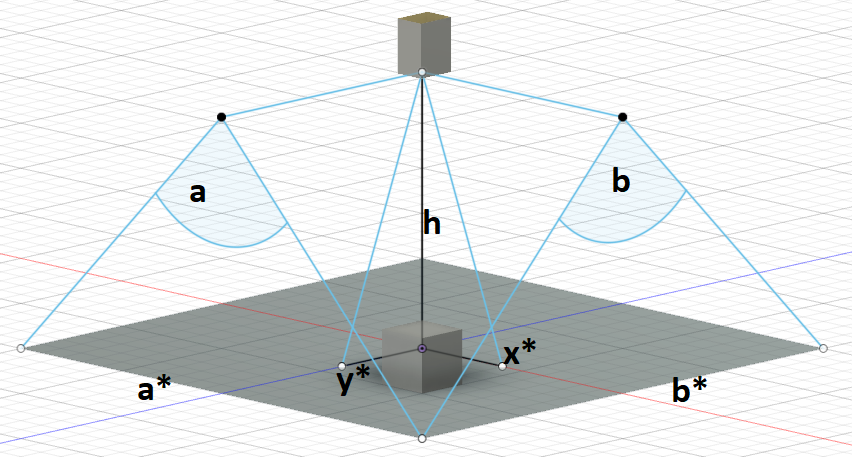
\includegraphics[scale=0.3]{"Grafiken/Kameraformel.png"}
	\caption{Kamerawinkel}
	\label{fig:meine-grafik}
\end{figure}
\section{Programmablauf}
Prinzipiell ist jede Node gleich aufgebaut. Zuerst gibt es eine Initialisierung und Verbindung mit der Masternode. Anschließend deklariert die Node welche Streams die entsprechende Node benötigt und welche nicht. Nun wird gewartet, bis eine neue Nachricht auftaucht und die diese wird dann verarbeitet. Geprüft wird in diesem Fall mit einer Rate von 20 Hz. \\
\\
Der Flight-Controller verhält sich jedoch leicht anders. Die PX-4 muss erst in den Offboard-Modus versetzt werden. Dieser bedeutet, dass die Drohne extern gesteuert werden kann. Außerdem muss der Arming-Modus aktiviert werden. Damit sie Befehle annimmt. Leider hat das einmalige Senden nicht gereicht. Sie hat nicht zuverlässig beide Befehle erkannt. Damit dies gewährleistet ist, sendet der Pi nun aller 5 Sekunden den Offboard Befehl, solange bis sich der Status der Drohne geändert hat, sodass sie sich nun im Offboardmodus befindet. Anschließend sendet der Controller das Arming Signal, solange bis die Drohne sich im Arming Modus befindet.\\
\\
Wichtig ist das gleichzeitig mit 20 Hz, eine Sollposition gesendet werden muss, damit die Drohne im nicht wieder aus dem Offboardmodus geht. Dies hat am Anfang große Probleme bereitet, da man so schnell die Kontrolle verliert.\\
\\
Anschließend wird zuerst eine Sollposition angeflogen. Aus dieser Position muss die Drohne, das Paket sehen. Anschließend richtet sich die Drohne mithilfe der Kamera mittig über dem Paket aus. Dabei vergleicht der Kontroller die aktuelle Position mit der Paketposition. Die Paketposition wird dabei mithilfe der Formel(siehe Sensorerfassung) berechnet. Anschießend wird es mit dem Faktor 10 dividiert, um sie langsam ausrichten zu lassen. Ist das Paket mittig und die Drohne nicht zu schnell(dies wird mithilfe der alten Position und der neuen Position bestimmt) so sinkt die Drohne. Hat sie eine Höhe von 60 cm erreicht, so dreht sie sich und richtet sich entlang des Paketes aus. Dabei verfährt sie nach dem gleichen Verfahren wie bei der Positionsausrichtung und wartet immer, bis das Paket wieder mittig ist. Ist die Verdrehung kleiner als 3 Grad, sinkt sie weiter. Ist sie nur noch 20 cm über dem Boden, so hat sie das Paket gefunden und schließt den Greifer. Anschließend könnte sie wieder abheben und das Paket zur Zielposition bringen. Der Prozess ist in dem unteren Strukturgramm dargestellt. 

\begin{figure}[h]
	\centering
	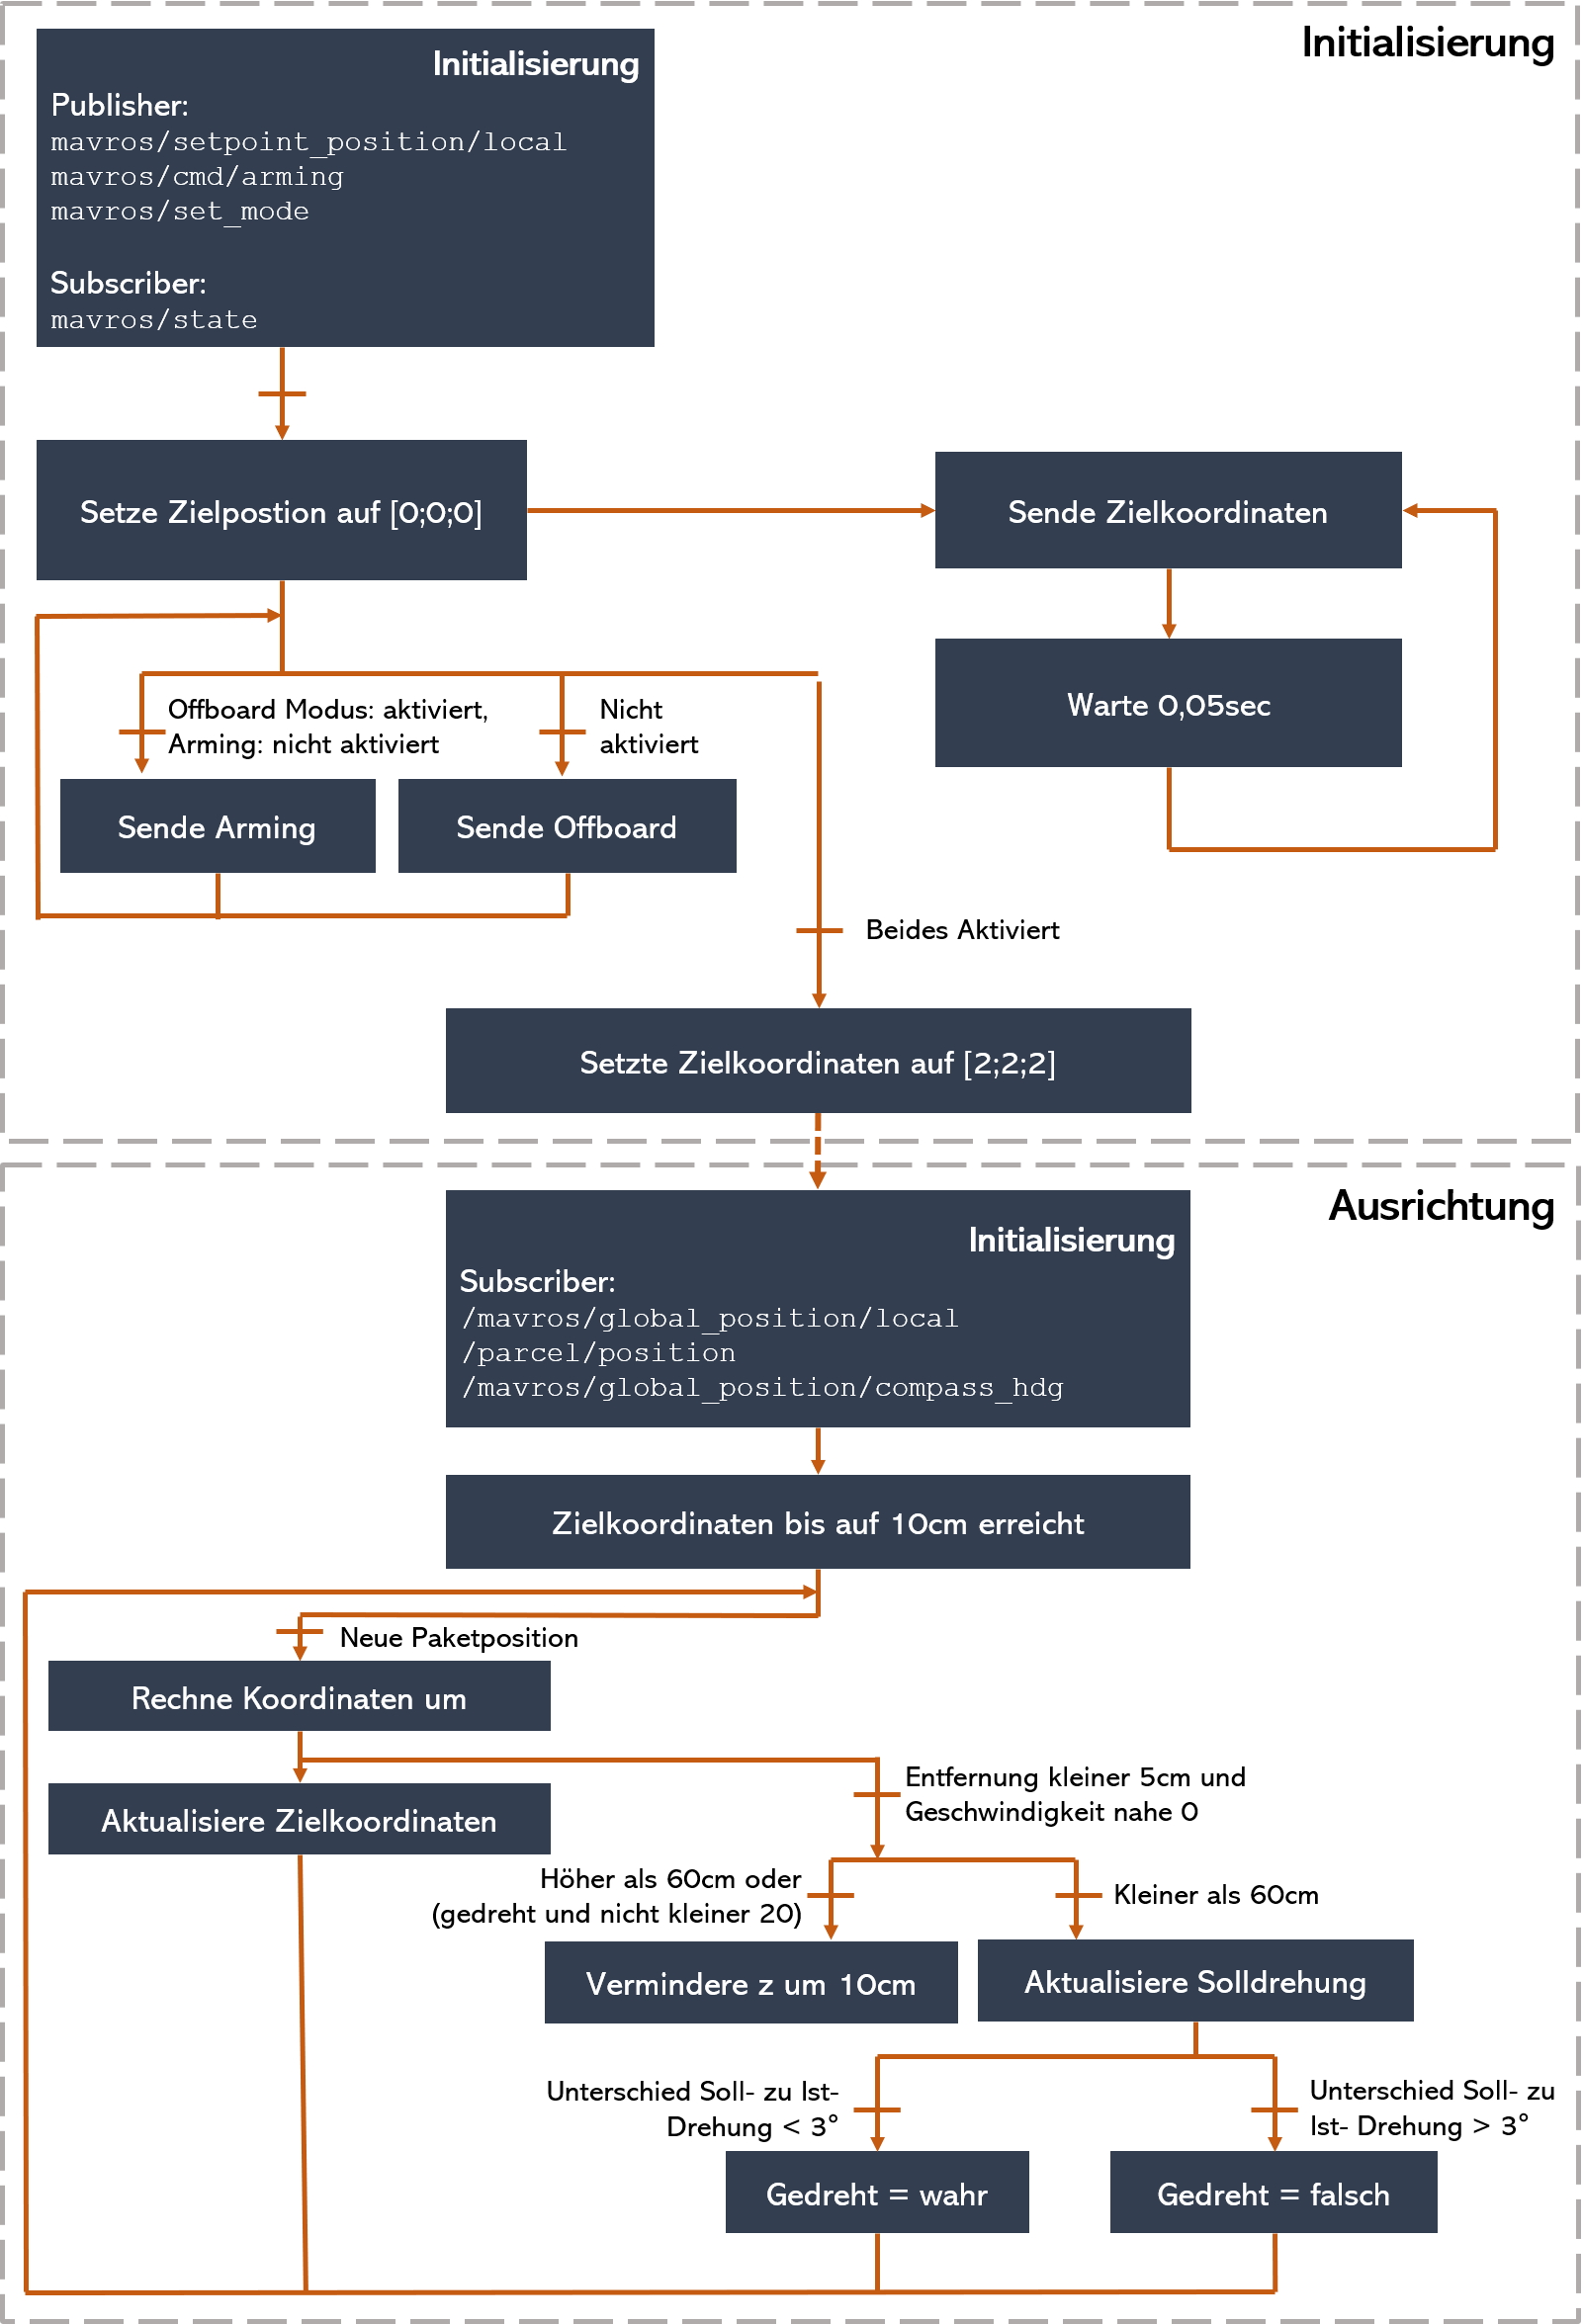
\includegraphics[scale=0.5]{"Grafiken/Prozellablauf.png"}
	\caption{Funktionsablaufdiagramm}
	\label{fig:meine-grafik}
\end{figure}